%% bare_conf.tex
%% V1.4a
%% 2014/09/17
%% by Michael Shell
%% See:
%% http://www.michaelshell.org/
%% for current contact information.
%%
%% This is a skeleton file demonstrating the use of IEEEtran.cls
%% (requires IEEEtran.cls version 1.8a or later) with an IEEE
%% conference paper.
%%
%% Support sites:
%% http://www.michaelshell.org/tex/ieeetran/
%% http://www.ctan.org/tex-archive/macros/latex/contrib/IEEEtran/
%% and
%% http://www.ieee.org/

%%*************************************************************************
%% Legal Notice:
%% This code is offered as-is without any warranty either expressed or
%% implied; without even the implied warranty of MERCHANTABILITY or
%% FITNESS FOR A PARTICULAR PURPOSE! 
%% User assumes all risk.
%% In no event shall IEEE or any contributor to this code be liable for
%% any damages or losses, including, but not limited to, incidental,
%% consequential, or any other damages, resulting from the use or misuse
%% of any information contained here.
%%
%% All comments are the opinions of their respective authors and are not
%% necessarily endorsed by the IEEE.
%%
%% This work is distributed under the LaTeX Project Public License (LPPL)
%% ( http://www.latex-project.org/ ) version 1.3, and may be freely used,
%% distributed and modified. A copy of the LPPL, version 1.3, is included
%% in the base LaTeX documentation of all distributions of LaTeX released
%% 2003/12/01 or later.
%% Retain all contribution notices and credits.
%% ** Modified files should be clearly indicated as such, including  **
%% ** renaming them and changing author support contact information. **
%%
%% File list of work: IEEEtran.cls, IEEEtran_HOWTO.pdf, bare_adv.tex,
%%                    bare_conf.tex, bare_jrnl.tex, bare_conf_compsoc.tex,
%%                    bare_jrnl_compsoc.tex, bare_jrnl_transmag.tex
%%*************************************************************************


% *** Authors should verify (and, if needed, correct) their LaTeX system  ***
% *** with the testflow diagnostic prior to trusting their LaTeX platform ***
% *** with production work. IEEE's font choices and paper sizes can       ***
% *** trigger bugs that do not appear when using other class files.       ***                          ***
% The testflow support page is at:
% http://www.michaelshell.org/tex/testflow/



\documentclass[conference]{IEEEtran}
% Some Computer Society conferences also require the compsoc mode option,
% but others use the standard conference format.
%
% If IEEEtran.cls has not been installed into the LaTeX system files,
% manually specify the path to it like:
% \documentclass[conference]{../sty/IEEEtran}


\IEEEoverridecommandlockouts 
\usepackage{macros}

\usepackage{amsmath}
\usepackage{blindtext, graphicx}
\usepackage{algorithm}

\usepackage{bbm}
\usepackage{soul}

\usepackage{algpseudocode}
\usepackage{pifont}
\usepackage{tikz}
\usepackage{amssymb}

\usepackage{upgreek}

\usepackage{mathtools}


% Some very useful LaTeX packages include:
% (uncomment the ones you want to load)


% *** MISC UTILITY PACKAGES ***
%
%\usepackage{ifpdf}
% Heiko Oberdiek's ifpdf.sty is very useful if you need conditional
% compilation based on whether the output is pdf or dvi.
% usage:
% \ifpdf
%   % pdf code
% \else
%   % dvi code
% \fi
% The latest version of ifpdf.sty can be obtained from:
% http://www.ctan.org/tex-archive/macros/latex/contrib/oberdiek/
% Also, note that IEEEtran.cls V1.7 and later provides a builtin
% \ifCLASSINFOpdf conditional that works the same way.
% When switching from latex to pdflatex and vice-versa, the compiler may
% have to be run twice to clear warning/error messages.






% *** CITATION PACKAGES ***
%
%\usepackage{cite}
% cite.sty was written by Donald Arseneau
% V1.6 and later of IEEEtran pre-defines the format of the cite.sty package
% \cite{} output to follow that of IEEE. Loading the cite package will
% result in citation numbers being automatically sorted and properly
% "compressed/ranged". e.g., [1], [9], [2], [7], [5], [6] without using
% cite.sty will become [1], [2], [5]--[7], [9] using cite.sty. cite.sty's
% \cite will automatically add leading space, if needed. Use cite.sty's
% noadjust option (cite.sty V3.8 and later) if you want to turn this off
% such as if a citation ever needs to be enclosed in parenthesis.
% cite.sty is already installed on most LaTeX systems. Be sure and use
% version 5.0 (2009-03-20) and later if using hyperref.sty.
% The latest version can be obtained at:
% http://www.ctan.org/tex-archive/macros/latex/contrib/cite/
% The documentation is contained in the cite.sty file itself.






% *** GRAPHICS RELATED PACKAGES ***
%
\ifCLASSINFOpdf
  % \usepackage[pdftex]{graphicx}
  % declare the path(s) where your graphic files are
  % \graphicspath{{../pdf/}{../jpeg/}}
  % and their extensions so you won't have to specify these with
  % every instance of \includegraphics
  % \DeclareGraphicsExtensions{.pdf,.jpeg,.png}
\else
  % or other class option (dvipsone, dvipdf, if not using dvips). graphicx
  % will default to the driver specified in the system graphics.cfg if no
  % driver is specified.
  % \usepackage[dvips]{graphicx}
  % declare the path(s) where your graphic files are
  % \graphicspath{{../eps/}}
  % and their extensions so you won't have to specify these with
  % every instance of \includegraphics
  % \DeclareGraphicsExtensions{.eps}
\fi
% graphicx was written by David Carlisle and Sebastian Rahtz. It is
% required if you want graphics, photos, etc. graphicx.sty is already
% installed on most LaTeX systems. The latest version and documentation
% can be obtained at: 
% http://www.ctan.org/tex-archive/macros/latex/required/graphics/
% Another good source of documentation is "Using Imported Graphics in
% LaTeX2e" by Keith Reckdahl which can be found at:
% http://www.ctan.org/tex-archive/info/epslatex/
%
% latex, and pdflatex in dvi mode, support graphics in encapsulated
% postscript (.eps) format. pdflatex in pdf mode supports graphics
% in .pdf, .jpeg, .png and .mps (metapost) formats. Users should ensure
% that all non-photo figures use a vector format (.eps, .pdf, .mps) and
% not a bitmapped formats (.jpeg, .png). IEEE frowns on bitmapped formats
% which can result in "jaggedy"/blurry rendering of lines and letters as
% well as large increases in file sizes.
%
% You can find documentation about the pdfTeX application at:
% http://www.tug.org/applications/pdftex





% *** MATH PACKAGES ***
%
%\usepackage[cmex10]{amsmath}
% A popular package from the American Mathematical Society that provides
% many useful and powerful commands for dealing with mathematics. If using
% it, be sure to load this package with the cmex10 option to ensure that
% only type 1 fonts will utilized at all point sizes. Without this option,
% it is possible that some math symbols, particularly those within
% footnotes, will be rendered in bitmap form which will result in a
% document that can not be IEEE Xplore compliant!
%
% Also, note that the amsmath package sets \interdisplaylinepenalty to 10000
% thus preventing page breaks from occurring within multiline equations. Use:
%\interdisplaylinepenalty=2500
% after loading amsmath to restore such page breaks as IEEEtran.cls normally
% does. amsmath.sty is already installed on most LaTeX systems. The latest
% version and documentation can be obtained at:
% http://www.ctan.org/tex-archive/macros/latex/required/amslatex/math/





% *** SPECIALIZED LIST PACKAGES ***
%
%\usepackage{algorithmic}
% algorithmic.sty was written by Peter Williams and Rogerio Brito.
% This package provides an algorithmic environment fo describing algorithms.
% You can use the algorithmic environment in-text or within a figure
% environment to provide for a floating algorithm. Do NOT use the algorithm
% floating environment provided by algorithm.sty (by the same authors) or
% algorithm2e.sty (by Christophe Fiorio) as IEEE does not use dedicated
% algorithm float types and packages that provide these will not provide
% correct IEEE style captions. The latest version and documentation of
% algorithmic.sty can be obtained at:
% http://www.ctan.org/tex-archive/macros/latex/contrib/algorithms/
% There is also a support site at:
% http://algorithms.berlios.de/index.html
% Also of interest may be the (relatively newer and more customizable)
% algorithmicx.sty package by Szasz Janos:
% http://www.ctan.org/tex-archive/macros/latex/contrib/algorithmicx/




% *** ALIGNMENT PACKAGES ***
%
%\usepackage{array}
% Frank Mittelbach's and David Carlisle's array.sty patches and improves
% the standard LaTeX2e array and tabular environments to provide better
% appearance and additional user controls. As the default LaTeX2e table
% generation code is lacking to the point of almost being broken with
% respect to the quality of the end results, all users are strongly
% advised to use an enhanced (at the very least that provided by array.sty)
% set of table tools. array.sty is already installed on most systems. The
% latest version and documentation can be obtained at:
% http://www.ctan.org/tex-archive/macros/latex/required/tools/


% IEEEtran contains the IEEEeqnarray family of commands that can be used to
% generate multiline equations as well as matrices, tables, etc., of high
% quality.




% *** SUBFIGURE PACKAGES ***
%\ifCLASSOPTIONcompsoc
%  \usepackage[caption=false,font=normalsize,labelfont=sf,textfont=sf]{subfig}
%\else
%  \usepackage[caption=false,font=footnotesize]{subfig}
%\fi
% subfig.sty, written by Steven Douglas Cochran, is the modern replacement
% for subfigure.sty, the latter of which is no longer maintained and is
% incompatible with some LaTeX packages including fixltx2e. However,
% subfig.sty requires and automatically loads Axel Sommerfeldt's caption.sty
% which will override IEEEtran.cls' handling of captions and this will result
% in non-IEEE style figure/table captions. To prevent this problem, be sure
% and invoke subfig.sty's "caption=false" package option (available since
% subfig.sty version 1.3, 2005/06/28) as this is will preserve IEEEtran.cls
% handling of captions.
% Note that the Computer Society format requires a larger sans serif font
% than the serif footnote size font used in traditional IEEE formatting
% and thus the need to invoke different subfig.sty package options depending
% on whether compsoc mode has been enabled.
%
% The latest version and documentation of subfig.sty can be obtained at:
% http://www.ctan.org/tex-archive/macros/latex/contrib/subfig/




% *** FLOAT PACKAGES ***
%
%\usepackage{fixltx2e}
% fixltx2e, the successor to the earlier fix2col.sty, was written by
% Frank Mittelbach and David Carlisle. This package corrects a few problems
% in the LaTeX2e kernel, the most notable of which is that in current
% LaTeX2e releases, the ordering of single and double column floats is not
% guaranteed to be preserved. Thus, an unpatched LaTeX2e can allow a
% single column figure to be placed prior to an earlier double column
% figure. The latest version and documentation can be found at:
% http://www.ctan.org/tex-archive/macros/latex/base/


%\usepackage{stfloats}
% stfloats.sty was written by Sigitas Tolusis. This package gives LaTeX2e
% the ability to do double column floats at the bottom of the page as well
% as the top. (e.g., "\begin{figure*}[!b]" is not normally possible in
% LaTeX2e). It also provides a command:
%\fnbelowfloat
% to enable the placement of footnotes below bottom floats (the standard
% LaTeX2e kernel puts them above bottom floats). This is an invasive package
% which rewrites many portions of the LaTeX2e float routines. It may not work
% with other packages that modify the LaTeX2e float routines. The latest
% version and documentation can be obtained at:
% http://www.ctan.org/tex-archive/macros/latex/contrib/sttools/
% Do not use the stfloats baselinefloat ability as IEEE does not allow
% \baselineskip to stretch. Authors submitting work to the IEEE should note
% that IEEE rarely uses double column equations and that authors should try
% to avoid such use. Do not be tempted to use the cuted.sty or midfloat.sty
% packages (also by Sigitas Tolusis) as IEEE does not format its papers in
% such ways.
% Do not attempt to use stfloats with fixltx2e as they are incompatible.
% Instead, use Morten Hogholm'a dblfloatfix which combines the features
% of both fixltx2e and stfloats:
%
% \usepackage{dblfloatfix}
% The latest version can be found at:
% http://www.ctan.org/tex-archive/macros/latex/contrib/dblfloatfix/




% *** PDF, URL AND HYPERLINK PACKAGES ***
%
%\usepackage{url}
% url.sty was written by Donald Arseneau. It provides better support for
% handling and breaking URLs. url.sty is already installed on most LaTeX
% systems. The latest version and documentation can be obtained at:
% http://www.ctan.org/tex-archive/macros/latex/contrib/url/
% Basically, \url{my_url_here}.




% *** Do not adjust lengths that control margins, column widths, etc. ***
% *** Do not use packages that alter fonts (such as pslatex).         ***
% There should be no need to do such things with IEEEtran.cls V1.6 and later.
% (Unless specifically asked to do so by the journal or conference you plan
% to submit to, of course. )


% correct bad hyphenation here
\hyphenation{Smart grids}

\begin{document}

%
% paper title
% Titles are generally capitalized except for words such as a, an, and, as,
% at, but, by, for, in, nor, of, on, or, the, to and up, which are usually
% not capitalized unless they are the first or last word of the title.
% Linebreaks \\ can be used within to get better formatting as desired.
% Do not put math or special symbols in the title.

\title{Smart Grid work for PES GM}


% author names and affiliations
% use a multiple column layout for up to three different
% affiliations

\author{A, B, C}
%\author{Raghuram$^\dagger$, D. Sai Koti Reddy$^\dagger$,  Shalabh Bhatnagar$^\dagger$
%\thanks{
%$^\dagger$ Department of Computer Science and Automation,
%Indian Institute of Science, Bangalore,
%E-Mail: danda.reddy@csa.iisc.ernet.in, shalabh@csa.iisc.ernet.in}
%}

%\author{\IEEEauthorblockN{Raghuram}
%\IEEEauthorblockA{Department of Computer Science and Automation\\
%Indian Institute of Science, Bangalore\\
%Bangalore, India \\
%Email: http://www.michaelshell.org/contact.html}
%\and
%\IEEEauthorblockN{D. Sai Koti Reddy}
%\IEEEauthorblockA{Department of Computer Science and Automation\\
%Indian Institute of Science, Bangalore\\
%Bangalore, India \\
%Email: danda.reddy@csa.iisc.ernet.in}
%\and
%\IEEEauthorblockN{Shalabh Bhatnagar}
%\IEEEauthorblockA{Department of Computer Science and Automation\\
%Indian Institute of Science, Bangalore\\
%Bangalore, India \\
%Email: shalabh@csa.iisc.ernet.in}
%}



% conference papers do not typically use \thanks and this command
% is locked out in conference mode. If really needed, such as for
% the acknowledgment of grants, issue a \IEEEoverridecommandlockouts
% after \documentclass

% for over three affiliations, or if they all won't fit within the width
% of the page, use this alternative format:
% 
%\author{\IEEEauthorblockN{Michael Shell\IEEEauthorrefmark{1},
%Homer Simpson\IEEEauthorrefmark{2},
%James Kirk\IEEEauthorrefmark{3}, 
%Montgomery Scott\IEEEauthorrefmark{3} and
%Eldon Tyrell\IEEEauthorrefmark{4}}
%\IEEEauthorblockA{\IEEEauthorrefmark{1}School of Electrical and Computer Engineering\\
%Georgia Institute of Technology,
%Atlanta, Georgia 30332--0250\\ Email: see http://www.michaelshell.org/contact.html}
%\IEEEauthorblockA{\IEEEauthorrefmark{2}Twentieth Century Fox, Springfield, USA\\
%Email: homer@thesimpsons.com}
%\IEEEauthorblockA{\IEEEauthorrefmark{3}Starfleet Academy, San Francisco, California 96678-2391\\
%Telephone: (800) 555--1212, Fax: (888) 555--1212}
%\IEEEauthorblockA{\IEEEauthorrefmark{4}Tyrell Inc., 123 Replicant Street, Los Angeles, California 90210--4321}}




% use for special paper notices
%\IEEEspecialpapernotice{(Invited Paper)}




% make the title area
\maketitle

% As a general rule, do not put math, special symbols or citations
% in the abstract
\begin{abstract}
This paper considers two important problems - on the supply-side and demand-side respectively and studies both in a unified framework. On the supply side, we study the problem of energy sharing among microgrids with the goal of maximizing profit obtained from selling power while meeting customer demand. On the other hand, under shortage of power, this problem becomes one of deciding the amount of power to be bought with dynamically varying prices. On the demand side, we consider the problem of optimally scheduling the time-adjustable demand - i.e., of jobs with flexible time windows in which they can be scheduled. While previous works have treated these two problems in isolation, we combine these problems together and provide for the first time in the literature, a unified Markov decision process (MDP) framework for these problems. We apply the Q-learning algorithm, a popular model-free reinforcement learning technique, to obtain the optimal policy. Through simulations, we show that our model outperforms the traditional power sharing models.



%In this paper, we consider two problems, one on the supply-side management another on the demand-side management of the smartgrid.
%%energy sharing among microgrids along with optimal scheduling of time adjustable smart home appliances demand. 
%On the supply-side, we study the problem of energy sharing among the microgrids with the goal of maximizing the profit obtained by selling the power while meeting the demand of its customers. Microgrids are equipped with a limited capacity batteries that can store the renewable energy. When they have excess power after meeting its demand, they need to take a decision on the amount of power to be sold and that to be stored in their batteries. This is a crucial decision to make as the renewable energy generation is uncertain in nature and the demand of its customers varies from time to time. A penalty is levied when the microgrid cannot satisfy the demand in any time instant. Similarly when there is a shortage of power, a decision needs to be taken on the amount of power to be bought. This decision is influenced by varying price of the power. Hence there is a control problem of taking the optimal decision on buying/selling the power in order to maximize its long term average profit.  
%
%On the demand-side, we consider the problem of optimally scheduling the time adjustable demand. These are the jobs that have a flexible time window in which they can be scheduled. Penalty is levied only if they are not scheduled at the end of their window. This allows us to intelligently schedule them so as to balance the load at the microgrid. For the first time, we combine these problems together and formulate them in a Markov Decision Process (MDP) framework. We apply a popular Reinforcement Learning algorithm Q-learning to provide solution to this problem. Through simulations, we show that our model outperforms the traditional power sharing models. 

 
%We formulate both the problems in a unified Markov decision process (MDP) framework for the first time to incorporate envisioned future smartgrid system.  We considered the infinite horizon average cost as objective function and used Q-learning algorithm at each microgrid. In simulations,
%we observed that our algorithms outperforms all the other algorithms by performing optimal choices for energy sharing and scheduling.






%One of the key challanges of Smart Grid management is ensuring to meet the demand while having control on the supply cost. 
%%\st{This concept of Smart Grid has become popular in the recent times. The main objective in this Smart Grid is to intelligently make use of power.} 
% It involves  performing optimal actions both at the production and consumption sites of  electric grid. In this work, we consider the problem of managing multiple microgrids attached to a central smart grid. Each of these microgrids are equipped with batteries to store renewable power.
% %\st{In this work, we consider multiple microgrids equipped with batteries to store renewable power}.
% At every instant, each of them receive a demand to meet. Depending on the supply (i.e., currently available battery energy, power drawn either from the central grid or from the peer microgirds), each of the microgrids take a decision on from where to draw the energy to meet the demand.
%% \st{Depending on the current battery and renewable power information, they take a decision on number of power units to be bought or sold.}
% When a microgrids buys energy either from the central grid or from the peer microgrids, it can use that energy either to meet the current demand or to store in the battery storage for future use. 
%%\st{If any of the other neighboring microgrids sell the power, they can consume it. Otherwise, they can get it from the main grid. If power is bought, it is first used to meet its demand and rest of it will be stored in the battery.}
% Hence, there is a control decision problem at each microgrid on the number of power units to be bought or sold at every time instant. We note that both the forecasted demand and predicted renewable supply impact this decision by each microgrid. 
%%\st{We note that the future forecast demand and renewable units also impact this decision.}
% Further, we consider some amount of the forecasted demand to be adjustable in terms of the time when it can be met by the microgrid. Such an adjustable demand is attributed due to the activities of daily living pertraining to Smart Homes connected to the microgrid networks. Hence, we formulate this problem in the framework of Markov Decision Process and apply Reinforcement Learning algorithms to solve this problem. Through simulations, we show that the policy we obtain performs an significant improvement over traditional techniques.
\end{abstract}

% no keywords

\section{Introduction} \label{sec:intro}

The smart grid is a distributed energy network composed of intelligent
nodes (or agents) that can either operate autonomously or communicate and share energy \cite{weiss1999multiagent}.
The purpose of a smart grid is to efficiently deliver energy to consumers as well as store and convert
energy produced, e.g., according to prices, supply and demand. 

A microgrid is a networked group of distributed energy sources with the goal of
generating, converting and storing energy. 
While the main power stations are highly connected, micro-grids with local power generation, storage
and conversion capabilities, act locally or share power with a few neighboring micro-grid nodes \cite{farhangi2010path}.
This scenario is being envisaged as an important alternative to the conventional scheme with
large power stations transmitting energy over long distances.

 In order to take full advantage of the modularity and flexibility of micro-grid technologies, smart
control mechanisms are required to manage and coordinate these distributed energy systems so as to
minimize the costs of energy production, conversion and storage, without jeopardizing grid stability.

The implementation of such smart controls is by no means easy for the following reasons:
\begin{inparaenum}[\bfseries (i)]
\item Small scale energy production and storage is intrinsically
         related to intermittency of wind/solar energy and to variability in the load profile.
          So an important challenge is to increase resilience and reliability under stochastic supply and
                 demand.
\item Micro-grids can operate in two different modes: (a) when they are connected to the
main power grid, and (b) in the isolated or island mode. Moreover, they can share energy with
other microgrids that require energy. Thus, one needs to make
dynamic decisions on (a) when to operate in the connected (to the power grid) or isolated modes, 
(b) when to share energy with other microgrids and when to store energy for future use, and (c) 
which form to store energy given that storage management itself
involves heterogeneous storage technologies with different
operating characteristics.
%\item Each microgrid has access to only its local (and not global) state information. 
%While microgrids can exchange information with one another, there are problems with frequent communication
%between microgrids due to (a) privacy issues and (b) risk of cyber attacks.
%Important challenges here include (a) optimizing global grid performance with limited communications,
%(b) voltage and frequency control for grid stabilization.
%\item Decision making in microgrids needs to take place on different timescales. On the slower
%timescale of say hours, one needs to make decisions on energy generation, conversion and storage,
%while on the faster timescale of minutes to seconds, one needs to make decisions related to dynamic
%demand response as well as ensuing grid stability, i.e., of frequency and voltage regulation.
\end{inparaenum}


%In this paper, we address two  problems. First,  energy sharing among the microgrids under stochastic supply and demand (mentioned above as (i) and (ii)) along with the optimal battery scheduling of a microgrid from the supply-side management (SSM) perspective. Second is from the demand-side management (DSM) perspective, which is efficiently scheduling the time adjustable demand from smart appliances in the smart home environment, called as an ADL (activity of daily living) demand along with the normal demand.  Our goal here is to reduce the energy demand and supply deficit in the long-run. We address this learning and scheduling problem by modeling them as a Markov decision process (MDP) \cite{puterman2014markov, vol2}.

In this paper, we address two  problems. (i) Supply-side management (SSM) problem: energy sharing among the microgrids under stochastic supply \& demand along with the optimal battery scheduling of each microgrid (ii) Demand-side management (DSM) problem: efficiently scheduling the time adjustable demand from smart appliances in the smart home environment along with the normal demand. Our goal here is to reduce the energy demand and supply deficit in the long-run. We address these learning and scheduling problems by modeling them as a Markov decision process (MDP) \cite{puterman2014markov}. 

%\begin{enumerate}[label={\bf\Roman*}]
\subsection{Supply-side management problem} \label{subsec:ssm}
 Supply-side management (SSM)\cite{} deals with developing techniques to  generate, transmit and distribute energy efficiently at supply-side. Cooperative energy exchange among microgrids is a popular technique in SSM for efficient energy distribution.  Local energy sharing/exchange between microgrids has the
following advantages:
(a) it can significantly reduce power wastage that would
otherwise result over long-distance transmission lines, and (b) it
helps satisfy demand and reduce reliance on the main grid. 
%Most importantly, energy exchange between microgrids needs to take place {\em with limited communication/information exchange}.
 Figure~\ref{gridmodel} shows a cooperative energy exchange model with multiple microgrids
(on the distribution side of the network) that can cater to their individual
local loads. Each microgrid controls its local sub-network through its controller (labelled
$\mbox{C}_1$, $\mbox{C}_2$ etc.) that mainly has access to its local state information.


\begin{figure}[thpb]
      \centering
      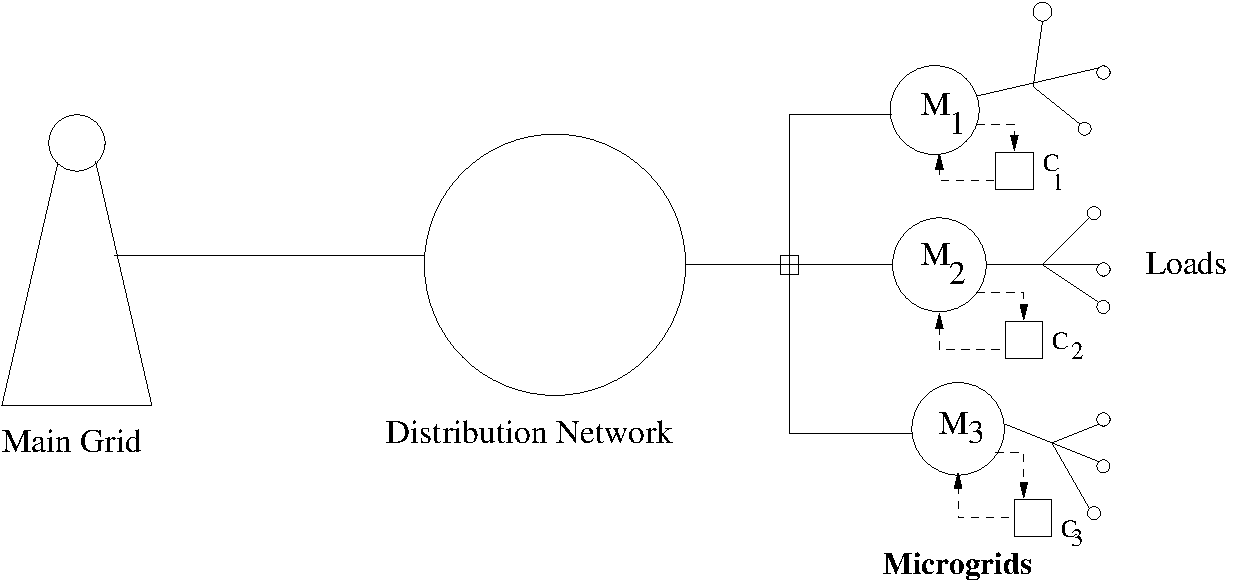
\includegraphics[scale=0.4]{powergrid2.pdf}
      \caption{Cooperative Energy Exchange Model}
      \label{gridmodel}
\end{figure}

 In classical power grids, system level optimization is done based on a centralized
objective function, where as 
microgrid network has heterogeneous nature right from the manner in which electricity
is generated such as from wind turbines, solar farms and diesel generators
to energy storage devices such as batteries and capacitors.
 Because of this heterogeneity and the fact that energy can be shared between microgrids depending
on requirements, one needs to consider asynchronous distributed techniques 
%such as multi-agent reinforcement learning or game theory
 to control and optimize a smart grid system
with a microgrid distribution network.



\textbf{Related work :} \cite{saad2012game} provides a survey on game theoretic approaches for microgrids where both cooperative energy sharing models as well as non-cooperative game models for distributed control of microgrids are examined when the system model is known. Since  models for energy dynamics are very unreliable \cite{zamora2010controls}, one has to use model-free algorithms to address these problems.  Because of their model-free nature, reinforcement learning \cite{sutton1998reinforcement} approaches that are primarily data-driven control techniques are playing a significant role in these problems.

In \cite{zifadistributed}, distributed reinforcement learning algorithm for coordinated energy sharing and voltage restoration in a islanded DC microgrid is proposed. In \cite{leo2014reinforcement}, reinforcement learning algorithm for optimal battery scheduling under the dynamic load environment and sloar power is proposed with the goal of  reducing  energy consumption from the main grid. In this paper, we  consider the coordinated energy sharing among the grid connected microgrids with optimal battery scheduling problem when stochastic supply and adjustable stochastic demand is available.

In \cite{pharsha}, authors consider the problem of optimal energy storage management under dynamic cost setup. They consider a renewable generator that is equipped with a limited storage battery and capable of meeting the some local demands. It also has connection from the main grid. The decision to be taken at every instant is the number of power units to be stored in the battery. They formulate this problem as a Markov Decision Process under long run average cost. The objective is to minimize the long run average cost of power bought from the main grid.


%****************** NEEDS TO BE CHANGED


%In \cite{PHarsha}, authors consider the problem of optimal energy storage management problem under dynamic cost setup. They consider a renewable generator that is equipped with a limited storage battery and capable of meeting the some local demands. It also has connection from the main grid. The decision to be taken at every instant is the number of power units to be stored in the battery. They allow this to be negative as power can be drawn from the battery. They formulate this problem as a Markov Decision Process under long run average cost. The objective is to minimize the long run average cost of power bought from the main grid.
%
%The assumption made in this paper is that demand at all times can be met. This is facilitated by allowing the main grid as many units of power as asked by the renewable generator. In our work, we extend this MDP model to put additional constraint on the maximum number of power units that a main grid can provide. Another notable contribution is that we extend this setup to the multiple microgrids. Here, we allow the microgrids to share the power among themselves.  

%In \cite{reddy2011learned}, they consider the problem of maximizing the profits among the broker agents. These agents buy the power from the producers and sell it to the customers. They apply Reinforcement Learning (RL) algorithms to solve this problem to show that learning policies perform better than the traditional non-learning strategies.

%In \cite{goodmdp}, authors propose an MDP for solving the problem of minimizing the demand and supply deficit  
%and apply dynamic optimization methods. But when the model information (the renewable energy generation in this case) is not known, we cannot apply these techniques.

%Demand side management (DSM) (\cite{logenthiran2011multi, wang2010demand,dsm1,dsm2,dsm3,dsm4}) deals with techniques developed to efficiently use the power by bringing the customers into the play. The main idea is to reduce the consumption of power during peak time and shifting it during the other times. This is done by dynamically changing the price of power and sharing this information with the customers. 

%*********************
\subsection{Demand-side management problem}\label{subsec:dsm}
 Load shifting is a popular technique used in demand-side management (DSM) \cite{DTU2010}. It involves moving the consumption of load to different times within an hour, or within in a day, or even within a week. It doesn't lead to reduction in net quantity of energy consumed, but simply involves changing the time when the energy is consumed. Advantage due to load shifting for the customer is reduction in the energy consumption cost, and the advantage for the smart grid is in managing the peak load consumption. Hence load shifting is beneficial for both the consumers and the smart grid.

With the increased use of the smart appliances and smart home environments, the concept of load shifting is becoming increasingly handy for the smart grid as the demand from smart appliances is time adjustable in general. One or more of these smart appliances collectively achieve some activity in the smart home environment, called as an ADL (activity of daily living). It's possible to monitor and identify the ADLs in the smart home environments \cite{I2014, GPG2016}. When an ADL is active, the smart appliances associated with that ADL are switched on to perform the activity defined by the ADL thus adding load on the smart grid. With the help of the smart home technology, it's possible to find the amount of load each ADL puts on the grid, and also the allowed time window during which the ADL would perform the activity (e.g., washing machine running for an hour to clean the cloths anytime between 3PM to 6PM). If the time window for the ADL lets the smart grid have more than one possible way of scheduling the load, it's considered as flexible ADL. On the other hand, if the time window for the ADL lets the smart grid have exactly one possible way of scheduling the load, it's considered as non-flexible ADL (e.g., washing machine running for an hour to clean the cloths anytime between 3PM to 4PM, is not flexible since there is only one option of switching on the washing machine at 3PM). Thus the demand from the flexible ADLs need not be met at a fixed time period, instead could be met at any time period within a flexible time window. With the help of the advanced metering infrastructure (AMI) \cite{RAFK2014} that provides a two-way communication between the utility and customers, it's possible to take the decision of when to schedule the ADL demand at the smart grid and convey the same to the customer's smart meter.    

There is other regular demand that needs to be met at fixed time periods, apart from the zero or more ADL related demand associated with any customer. This regular demand along with the zero or more non-flexible ADL demand of a smart home is considered to be non-ADL demand for the rest of the paper. Similarly, the demand due to zero or more flexible ADLs of the smart home is considered to be ADL demand.
 
There is prior art around scheduling the ADL-demand using the load shifting technique for handling the peak load scenarios \cite{CL2014}. However, they precisely know the supply profile while doing such a scheduling of the ADL-demand. In this paper, we propose scheduling of ADL-demand using the load shifting technique with uncertainty in the supply profile generated (e.g., renewable energy sources like solar or wind being the primary sources of power generation).

\textbf{Our contributions :}
\begin{inparaenum}[\bfseries (i)]
We summarize our contributions as follows :\\
\item To the best of out knowledge, we are the first one to integrate both the Demand-side and Supply-side management problems  in a single Markov decision process framework. We used reinforcement learning algorithms which do not require knowledge of the underlying model to address these problems. Our algorithms are easy to implement and also scalable.\\
\item The Optimal scheduling of ADL demand at microgrid level, where both the demand and power generation is stochastic is first time introduced through this work. \\    
\end{inparaenum}

The rest of the paper is organized as follows. In the section \ref{sec:model}, we discuss in detail about the problem formulation using MDP framework. We present  in section \ref{sec:algo} about our Q-learning algorithm. In section \ref{sec:experiments}, we present simulation experiments along with other algorithms for comparison. Finally in section \ref{sec:conclusion}, we provide the concluding remarks.


% For peer review papers, you can put extra information on the cover
% page as needed:
% \ifCLASSOPTIONpeerreview
% \begin{center} \bfseries EDICS Category: 3-BBND \end{center}
% \fi
%
% For peerreview papers, this IEEEtran command inserts a page break and
% creates the second title. It will be ignored for other modes.
\IEEEpeerreviewmaketitle



 


% \subsection{Subsection Heading Here}
% Subsection text here.


% \subsubsection{Subsubsection Heading Here}
% Subsubsection text here.

%\section{Problem and Model}

Consider multiple microgrids deployed at the sites where renewable energy is available. They are provided with the limited storage batteries that can store the power. Note that they do not have power generation capabilities. They have electrical connections from neighboring microgrids and also from the main grid. But the sharing of power among the microgrids is the most preferred mode as it results in the minimum dissipation loss of power. Only if the sharing among the microgrids is not possible, the main grid connection comes into play. 

At the beginning of every time instant (For ex. every hour of a day), each microgrid obtains the demand that they need to meet. They also obtain the renewable power generated in that instant. Based on these two information, along with the battery information, the microgrids need to take a decision on number of power units to be bought/sold. If the power is bought, it is first used to meet the demand and the remaining will be stored in the battery. One may think of a simple greedy policy to solve this problem. That is, the microgrids sells the excess units and buys when there is deficit of demand. But this behaviour may not result in the optimal behavior in a long-run. For example, consider a situation where a microgrid have an surplus of power. But the forecasted demand in the future is very high and the forecasted renewable energy is very low. In this case, having power in its battery will be very helpful. Otherwise, it has to buy the power from the main grid which can be very high. Hence the microgrid needs to balance the current and future rewards. Mathematically, we can formulate this problem in the framework of Markov Decision Process (MDP).

*** Write about MDP, Infinite horizon and Average cost MDP *******

Now we formally present the MDP model for our problem. Let us denote $x_{t}^{i} = (d_{t}^{i},r_{t}^{i},b_{t}^{i})$  as the demand, renewable generation and battery information of the microgrid $i$ at time instant $t$. Let the maximum size of the battery be $B$. We assume that the Demand is a Markov Process. That is, the demand in the next time period depends only on the current demand. Renewable generation is assumed to be a stochastic process. As described earlier, the microgrids can share the power among themselves. This is done at the price decided by the main grid. We denote the price of a unit of power at time instant $t$ as $p_{t}$. The price is also modeled as a Markov Process. Thus the state space is denoted by $s_{t}^{i} = <t,x_{t}^{i},p_{t}>$. Note that we include the current time also in the state space. This is because for the same $x_{t}^{i}$ and $p_{t}$, the decision taken can be different at different times. For example, a microgrid operating on solar renewable will be able to sell the power during the morning time as they may still receive the solar power during the afternoon. But they may not want to sell the power during the evening as they will be no solar power in the night. Instead they store the excess power in the battery.

The decision taken by the microgrid $i$ at the time $t$ is denoted as $u_{t}^{i}$. This can be positive or negative. Positive action denotes the number of units that the microgrid is willing to sell. Negative units represents the number of units that the microgrid is willing to buy. If a microgrid needs power, it first accepts it from the neighboring microgrids. Then the remaining units (if any) will be bought from the main grid. If any microgrid has a surplus power that is not consumed by any other, it sells it to the main grid. To maintain the stability at the main grid, We impose a constraint on the number of units of power $M$ that a main grid can give to each microgrid. 

We observe that the action to be taken depends only on the net demand. That is we can further simplify the state space to be $s_{t}^{i} = (t,nd_{t}^{i},p_{t})$ where $nd_{t}^{i} = r_{t}^{i} + b_{t}^{i} - d_{t}^{i}$. If this is negative, it means there is a deficit in demand and positive implies there is excess of power.

Then the action is bounded as follows. For ease of understanding, we drop the subscripts.  

\begin{align}
-min(M, B - nd) \leq u \leq max(0, nd)
\end{align}

The intuition behind the bounds is as follows. A microgrid can sell atmost the excess power. That is, the power remaining after meeting the demand. While buying, it can buy to meet the demand and also to fill its battery.

The battery information is updated as follows:

\begin{align}
b_{t+1}^{i} = max(0,nd_{t}^{i} - u_{t}^{i})
\end{align}

We formulate the single stage cost function as follows :
\begin{align}
g^{i}(s,u) = p_{t}*u_{t}^{i} + c*(min(0,nd_{t}^{i} - u_{t}^{i}).
\end{align}

The first term represents the cost of buying or selling the power and the second term represents the demand and supply deficit. For every unit of demand that is not met, the microgrid incurs a cost of $c$. 

Finally, the objective of the microgrid $i$ is to maximize the following \cite{avgcost}:

\begin{align}
limsup_{n \rightarrow \infty} 1/n \sum_{k = 0}^{n} E(g^{i}(s_{k},u_{k})),
\end{align}

where $E(.)$ is the expectation. 

We also consider the long run discounted cost formulation. The objective here is to maximize the following:

\begin{align}
limsup_{n \rightarrow \infty} \sum_{k = 0}^{n} \gamma^{k} * E(g^{i}(s_{k},u_{k})),
\end{align}

where $\gamma$ is the discount factor. 
\section{Problem formulation and mdp model} \label{sec:model}
%Microgrids comprise of the distributed small scale power generating sources, mainly renewable energy sources (mainly wind and solar ) and  are also equipped with storage devises.
We consider $N$ microgrids denoted by $\{1,\ldots,N\}$, which are inter-connected through distribution network. In this paper, we consider the case when microgrids are connected  to the main grid (i.e, they are operated in grid connected mode). Each microgrid comprise of the distributed small scale renewable power generating sources and also equipped with energy storage devices. Let $B_i$ be the maximum energy storage capacity of microgrid $i$. At every time step $t$ of a day, $i$th microgrid controller $C_i$ is having the following information:
\begin{enumerate}[label=(\alph*)]
\item Total generated energy from all its distributed renewable energy sources denoted by  $r_t^i$.
% (super script $i$ used to refer to microgrid $i$).
\item Accumulated non-ADL demand denoted by $d_t^i$, from each load in the $i$th microgrid. 
\item Set of all ADL jobs at microgrid $i$ denoted $J_{t}^{i}$.  $J_{t}^{i}$ is of the form $\{\gamma_{1}^{i},\ldots,\gamma_{n}^{i}\}$, where $j$th ADL job $\gamma_{j}^{i}$, is a tuple consists of  number of units of energy required to finish that job denoted by $a_{j}^{i}$ and an integer  $f_{j}^{i}$, which denotes number of future time slots remaining by which one can schedule that job without incurring the penalty. Let  it be represented as follows $\gamma_{j}^{i} = (a_{j}^{i}, f_{j}^{i})$. Let the total ADL demand be denoted by $A_t^i= \sum_{j=1}^{n} a_j^i$.
\item  Total energy available in the storage device of microgrid $i$, denoted by $b_{t}^{i}$.
\end{enumerate} 
In this paper, we are considering the cooperative energy exchange model under which microgrids can share energy among themselves. 
From the above available information, microgrid controller  $C_i$ at every time step $t$ has to decide on the following choices: (a)  Amount of energy it needs to buy/sell from the main grid, (b) Amount of energy it needs to buy/sell from the neighboring microgrids,
(c) Amount of the energy it needs to store/take from the storage device, and (d) Sub-set of ADL jobs it needs to schedule. Both the demand and energy generated at microgrid $i$ is uncertain/random due to  random nature of  loads ($d_t^i$ and $A_t^i$) and renewable energy generation ($r_t^i$). 

Markov decision process (MDP)  is a general framework for modeling problems of dynamic optimal decision making under uncertainty. *****Need to write about MDP*******.
%We modeled our problem in the framework of MDP. 
 In the next sub-section we provide the details of our MDP model.
\subsection{MDP framework}
\subsubsection{State space}
The state $s_{t}^{i}$ at time instant $t$  for microgrid $i$ is as follows:
\begin{align}
s_{t}^{i} = (t,nd_{t}^{i},p_{t}, J_{t}^{i}),
\end{align}
where the net demand $nd_{t}^{i} = r_{t}^{i} + b_{t}^{i} - d_{t}^{i}$, which denotes whether there is an excess power or deficit.  And $p_{t} and  J_{t}^{i}$ denotes the price per unit energy and set of all ADL jobs at time instant $t$ respectively. If  net demand $nd_{t}^{i}$ is positive then it implies that there is excess of power after meeting the non-ADL demand and if negative implies that there is a deficit in power even to meet the non-ADL demand. Current time slot is  included in the state since optimal action can depend on time. For example, microgrid operating on solar renewable generation can sell any excess power during the morning as the solar power will be available even during afternoon. But it may not be an optimal decision to sell in the evening as there will be no solar power during the night. 
\subsubsection{Action space}
At each time instant $t$ microgrid controller needs to take two decision $u_{t}^{i}$ and $v_{t}^{i}$. The first action $u_{t}^{i}$, if positive, denotes the number of units that the microgrid is willing to sell and if negative, represents the number of units that the microgrid is willing to buy. The second action $V_{t}^{i}$ pertains to the scheduling decision of ADL jobs taken by microgrid $i$.

Let $P_{t}^{i}$ be the power set of $J_{t}^{i}$, which consists of all possible combinations of the ADL jobs that can be scheduled at time instant $t$ at microgrid $i$. Let  $A_{t}^{i}$ consists of the total aggregated demand  for every subset in  $P_{t}^{i}$. For example, let the $j$th element of $A_{t}^{i}(j) = \sum_{k=1, \gamma_k^i \in P_{t}^{i}(j) }^n a_k^i$, where $ P_{t}^{i}(j)$ is $j$th element of  $P_{t}^{i}$.
%Let $P_{t}^{i} = \{\Gamma_{1}^{i},\ldots,\Gamma_{N}^{i}\}$ be the power set of $J_{t}^{i}$, which consists of all possible combinations of the ADL jobs that can be sheduled at time instant $t$ at microgrid $i$. 
%Let  $A_{t}^{i} = \{A(\Gamma_{1}^{i}),\ldots,A(\Gamma_{N}^{i})\} $, where $A(\Gamma_{j}^{i}) = \sum_{\gamma_{k}^{i} \in \Gamma_{j}^{i} } a_{k}^{i}$.
 The feasible region for action $u_{t}^{i}$ is bounded as follows:
\begin{align}
-min(M_t^i, B_t^i - nd_t^i + &\max_{1\leq j \leq 2^n} A(j) ) \leq u_t^i \nonumber\\ &\leq max(0, nd_t^i - \min_{1\leq j \leq 2^n} A(j)),
\end{align}
where $M_t^i$ denotes maximum amount of power main grid can give it to microgrid $i$. This constraint is to maintain stability of the main grid. Above bounds represents the following, microgrids can sell the power only after meeting its non-ADL demand and can buy to fill its battery after meeting its both ADL and non-ADL demands.
%The intuition behind the bounds is as follows. A microgrid can sell atmost the excess power. That is, the power remaining after meeting the demand. While buying, it can buy to meet the demand and also to fill its battery.

After controller picks action $u_{t}^{i}$, we construct the feasible set $F_{t}^{i}$, which is a subset of $P_{t}^{i}$. It consists of all possible subsets of ADL jobs that can be scheduled with $u_{t}^{i}$. More formally, each element $j$ of  $F_{t}^{i}$ has to satisfy the following condition :   $A_t^i(j) \leq u_{t}^{i} $, where $A_t^i(j)$ is total energy required to finish all the ADL jobs in it. Now, controller picks action $v_{t}^{i}$ which is an element in $F_{t}^{i}$, which results in scheduling all the ADL jobs in that subset. The remaining power is used to meet the non-ADL demand and for storing in the battery for future use.

%Each element $\Gamma_{j}^{i}$ in the $F_{t}^{i}$ has to satisfy the following condition $A(\Gamma_{j}^{i}) \leq u_{t}^{i} $.
%Agent has to pick the action $v_{t}^{i} = \Gamma_{j}^{i} \in F_{t}^{i}$. Now ADL jobs in $\Gamma_{j}^{i}$ will get sheduled. 
 Let $\widehat J_{t+1}^{i}$ be the new set of ADL jobs received by controller at time instant $t+1$. Depends on action $v_{t}^{i}$, some of the ADL jobs will not get scheduled. We pass them to time step $t+1$, if they can be scheduled without incurring the penalty. The set of all ADL jobs at time instant $t+1$ is union of the new ADL jobs and old ADL jobs which are not scheduled after reducing there  $f_{j}^{i}$ by one ( number of future time slots remaining by which one can schedule that job without incurring the penalty) .
%For the next time instant $t+1$, we update the following :
$J_{t+1}^{i} = \widehat J_{t+1}^{i} \cup \widetilde J_{t}^{i}$, where $\widetilde J_{t}^{i} =  \{(a_{1}^{i}, f_{1}^{i} - 1),\ldots,(a_{n}^{i}, f_{n}^{i} - 1)\}$, and $ (a_{j}^{i}, y_{j}^{i}) \in \overline J_{t}^{i}$. And $\overline J_{t}^{i} = J_{t}^{i} - v_{t}^{i}$.

The storage device battery information is updated as follows:
\begin{align}
b_{t+1}^{i} = max(0,nd_{t}^{i} - u_{t}^{i}),
\end{align}
which denotes the power available after meeting the non-ADL demand and ADL demand is stored in the battery for future use.
\subsubsection{Single stage reward function}
In this paper, we want to maximize the profit of each microgrid obtained by selling power while reducing the demand and supply deficit. Our singe stage reward function has both the reward obtained by selling power and penalty for unmet demand. The single stage reward  function for our MDP is as follows :
\begin{align}
g_t^{i}(s_t^i,u_t^i) = p_{t}*u_{t}^{i} + c*(min(0,&nd_{t}^{i} - u_{t}^{i}))  \nonumber\\ &+ c* \sum_{k =1}^{n} I_{f_{k}^{i} = 0} a_{k}^{i} ,
\end{align}
The first term represents the cost/gain incurred for  buying/selling the power, and the second and third terms represents the penalty  incurred for not meeting the non ADL demand and ADL demand respectively. Here, $c$ is penalty per unit of unmet demand and $I_{f_{k}^{i}}$ is indicator random variable which is equal to one if $f_{k}^{i} =0$ and zero otherwise. 
%The microgrid incurs a cost of $c$ for every unit of demand that is not met. 
******Need to write about transition probability kernel ***********.
\subsection{Average cost setting}
Finally, the objective of the microgrid $i$ is to maximize the following \cite{avgcost}:
\begin{align}
limsup_{n \rightarrow \infty} 1/n \sum_{k = 0}^{n} E(g^{i}(s_{k},u_{k})),
\end{align}
where $E(.)$ is the expectation. 

We also consider the long run discounted cost formulation. The objective here is to maximize the following:

\begin{align}
limsup_{n \rightarrow \infty} \sum_{k = 0}^{n} \gamma^{k} * E(g^{i}(s_{k},u_{k})),
\end{align}

where $\gamma$ is the discount factor. 

%%%%%%%%%%%%%%%%%%%%%%%%%%%%%%%%%%%%%%%%%%%%%%%%%%%%%%%%%%%%%%%%%%%%%%%%%%%%%%%%%%%%%%%
%%%%%%%%%%%%%%%%%%%%%%%%%%%%%%%%%%%%%%%%%%%%%%%%%%%%%%%%%%%%%%%%%%%%%%%%%%%%%%%%%%%%%%%
%\algblock{PEval}{EndPEval}
%\algnewcommand\algorithmicPEval{\textbf{\em Function evaluation 1}}
% \algnewcommand\algorithmicendPEval{}
%\algrenewtext{PEval}[1]{\algorithmicPEval\ #1}
%\algrenewtext{EndPEval}{\algorithmicendPEval}
%
%\algblock{PEvalPrime}{EndPEvalPrime}
%\algnewcommand\algorithmicPEvalPrime{\textbf{\em Function evaluation 2}}
% \algnewcommand\algorithmicendPEvalPrime{}
%\algrenewtext{PEvalPrime}[1]{\algorithmicPEvalPrime\ #1}
%\algrenewtext{EndPEvalPrime}{\algorithmicendPEvalPrime}
%
%\algblock{PImp}{EndPImp}
%\algnewcommand\algorithmicPImp{\textbf{\em Gradient descent}}
% \algnewcommand\algorithmicendPImp{}
%\algrenewtext{PImp}[1]{\algorithmicPImp\ #1}
%\algrenewtext{EndPImp}{\algorithmicendPImp}
%
%\algtext*{EndPEval}
%\algtext*{EndPEvalPrime}
%\algtext*{EndPImp}
%%%%%%%%%%%%%%%%% alg-custom-block %%%%%%%%%%%%
%\algblock{PEvalPrimeDouble}{EndPEvalPrimeDouble}
%\algnewcommand\algorithmicPEvalPrimeDouble{\textbf{\em Function evaluation 3}}
% \algnewcommand\algorithmicendPEvalPrimeDouble{}
%\algrenewtext{PEvalPrimeDouble}[1]{\algorithmicPEvalPrimeDouble\ #1}
%\algrenewtext{EndPEvalPrimeDouble}{\algorithmicendPEvalPrimeDouble}
%\algtext*{EndPEvalPrimeDouble}
%
%\algblock{PImpNewton}{EndPImpNewton}
%\algnewcommand\algorithmicPImpNewton{\textbf{\em Newton step}}
% \algnewcommand\algorithmicendPImpNewton{}
%\algrenewtext{PImpNewton}[1]{\algorithmicPImpNewton\ #1}
%\algrenewtext{EndPImpNewton}{\algorithmicendPImpNewton}
%
%\algtext*{EndPImpNewton}
%
%%%%%%%%%%%%%%%%%%%%
%
%\begin{algorithm}[t]
%\begin{algorithmic}
%\State {\bf Input:} 
%initial parameter $x_0 \in \R^N$, perturbation constants $\delta_n>0$, step-sizes $\{a_n, b_n\}$, operator $\Upsilon$.
%\For{$n = 0,1,2,\ldots$}	
%	\State Generate $\{d_n^{i}, i=1,\ldots,N\}$, independent of $\{d_m, m=0,1,\ldots,n-1\}$. 
%	\State For any $i=1,\ldots,N$, $d_n^{i}$ is distributed either as an asymmetric Bernoulli (see \eqref{eq:det-proj}) or Uniform $U[-\eta,\eta]$ for some $\eta >0$ (see Remark \ref{remark:unif}). 
%	\PEval
%	    \State Obtain $y_n^+ = f(x_n+\delta_n d_n) + \xi_n^+$.
%  \EndPEval
%	    \PEvalPrime
%	    \State Obtain $y_n^- = f(x_n-\delta_n d_n) + \xi_n^-$.
%	    \EndPEvalPrime
%	    	    \PEvalPrimeDouble
%	    \State Obtain $y_n = f(x_n) + \xi_n$.
%	    \EndPEvalPrimeDouble
%	    \PImpNewton
%		\State Update the parameter and Hessian as follows:
%		\begin{align*}
%		x_{n+1} = & \; x_n - a_n \Upsilon(\overline H_n)^{-1}\widehat\nabla f(x_n), \\
%\overline H_n = &\; (1-b_{n})  \overline H_{n-1} + b_{n} ( \widehat H_n - \widehat \Psi_n),
%\end{align*}
%where $\widehat H_n$ and $\widehat \Psi_n$ are chosen according to \eqref{eq:2rdsa-estimate-ber} and \eqref{eq:psinhat}, respectively. 
%		\EndPImpNewton
%\EndFor
%\State {\bf Return} $x_n.$
%\end{algorithmic}
%\caption{Structure of 2RDSA-IH algorithm.}
%\label{alg:structure}
%\end{algorithm}

\section{Algorithm}\label{sec:algo}

%We first note that the renewable generation is uncertain in nature. 
%That is, we do not know in the current time period, the renewable generation in the future time periods.

 In this paper, we do not assume any model of the system (probability transition model of the demand, supply and reward structure) due to uncertainity of renewable energy generation. We employ RL agorithms which does not assume any model to provide optimal solution.

We employe Q-Learning algorithm, a  popular RL method for solving the average cost probelm in \ref{subsec:avg}.
%To solve the above average cost problem, we apply a popular RL algorithm, Q-Learning.
 Our objective is to obtain a stationary optimal policy $\pi : S \rightarrow A$, which is a mapping from state to the action space.  
We apply the Relative Value Iteration (RVI) based Q-Learning described in \cite{avgcost}. In this algorithm, we update the Q-values in each iteration according to the following rule:
\begin{align}
Q^{n+1}(&s,u) = Q^{n}(s,u) + \alpha(n)(g(s,u,s^{'}) + \nonumber\\ &  max_{u} Q^{n}(s^{'},u) - max_{u} Q^{n}(s_{0},u) - Q^{n}(s,u)),
\end{align}
where $\alpha$ is the learning rate and $s_{0}$ is any prescribed state.
The $Q^n(s,u)$ represents the $n$th estimate of the Q-value  obtained in state $s$ by taking an action $u$. In \cite{avgcost}, it is shown that under appropriate learning rate, the algorithm converges to the  optimal policy. 
Each microgrid will run the algorithm independently until convergence. Then the optimal policy of microgrid $i$ is obtained as follows
\begin{align}
\pi_{i}^{*}(s) = max_{u}Q^{i}(s,u),
\end{align}
that is, the optimal policy in state $s$ is selected by taking the maximum over all actions of the Q-values.  


\section{Simulation Experiments}
We implemented our models on network with 3 microgrids. Two microgrids are operating on solar renewable generation and the other on wind renewable energy. To simulate the renewable generation, we use RAPsim software \cite{rapsim}. RAPsim is an open source simulator for analyzing the power flow in microgrids. It has a provision for simulating the renewable generation, which is the main feature that we use in our experiments. We construct our microgrid model as shown in the figure. We can see that there are three microgrids, two of them operating on the solar energy and the other on the wind energy. They also have electrical connections from the main grid. Each microgrid provides power to the respective houses on their power line. 

\subsection{Implementation}

We implement the model we described in the section 2. We call this model as $ADL-sharing$ model. For comparison purposes, we implement following models. 

\begin{itemize}
	\item \textbf{Greedy-ADL model}: In this model, the microgrids will exhibit the greedy behavior. They share the power only if there is excess power after filling up the battery. That is, the action in each instant is bounded by   
	
	\begin{align}
	-min(M, B - nd) \leq max(0,nd - B) 
	\end{align}
	
	That is, if the net demand is negative, decision is taken on amount to power to buy to meet the demand and fill the battery. On the other hand, if the net demand is positive, it is first used to fill the battery and only if there is any excess power left, it will be sold to other microgrids.
	
	\item \textbf{Non-ADL model}:  This model is similar to the $ADL-sharing$ model, but without the integration of ADL demand. In this model, the ADL demand is added to the main demand. Unlike the $ADL-sharing$ model, there is no flexibility of intelligently scheduling the ADL demand. 
	
\end{itemize}

\subsection{Setup}

% \begin{figure}
%still need the trimming of figure. include when we put experimental figures
% 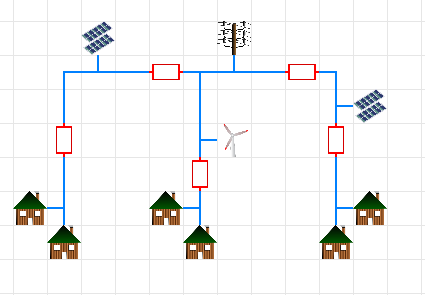
\includegraphics[scale = 0.4]{experimental_setup.jpg}
% \end{figure}

We simulate the above setup for the month of September 2017 and collect the wind and solar renewable power generated each day every hour. The parameters for our experiments are described below. The number of decision time periods is taken to be 4. We consider 3 demand values for all the microgrids - 2, 4 and 6 units. The probability transition matrices for all the 3 microgrids are given below :


\[
P_{1}=
\begin{bmatrix}
0.2 & 0.6 & 0.2 \\
0.1 & 0.2 & 0.7 \\
0.8 & 0.1 & 0.1
\end{bmatrix}
\]

\[
P_{2}=
\begin{bmatrix}
0.2 & 0.2 & 0.6 \\
0.8 & 0.1 & 0.1 \\
0.2 & 0.7 & 0.1
\end{bmatrix}
\]

\[
P_{3}=
\begin{bmatrix}
0.5 & 0.5 & 0 \\
0 & 0.5 & 0.5 \\
1 & 0 & 0
\end{bmatrix}
\]




The price values is considered to be 5, 10 and 15. The Probability transition matrix for the price vector is given below:



\[
Q=
\begin{bmatrix}
0.2 & 0.4 & 0.4 \\
0.1 & 0.5 & 0.4 \\
0.5 & 0.4 & 0.1
\end{bmatrix}
\]


Maximum size of battery and maximum renewable power generated is taken to be 8 units. The maximum power that a microgrid can obtain from the main grid is set to 10 units.

We consider 3 ADLs in our experiment. First ADL requires 1 unit of power that needs to be satisfied within the second time period. Second ADL requires 1 unit of power within the third time period. Third ADL requires 2 units of power within the fourth time period.

With this setup, we compare our proposed models. The algorithms are trained for $10^6$ iterations. For comparison purposes, we plot value of threshold $c$ on X-axis and Average reward on Y-axis. Average reward is computed as follows. We run the trained models for 1000 runs and average the reward obtained by each microgrid. 

\subsection{Observations}

\subsection{Discussion}

In Figure 1, we compare our $ADL-sharing$ model with the $Greedy- ADL$. As discussed earlier, in the latter model the sharing of power is done only when there is excess after filling the battery. We can see that the first model outperformed the second model. Even though there will be less buying of power in $Greedy-ADL$, there will be no selling of power as well. Therefore  the overall profit obtained will not be higher than that, when the intelligent decisions are made. Hence we can conclude that the intelligent sharing of power among microgrids yields more profit than that of the non-sharing case. 

In Figure 2, we compare our $ADL-sharing$ model with the $Non-ADL$ model. We can observe from the plot that, our model 1 outperforms the model 3. The reason for that is discussed below. Consider $c \geq 15$, which is the maximum price. In $ADL-sharing$, there is a flexibility to intelligently schedule the ADL activities according to the non-ADL demand and price. But this is not the case with the $Non-ADL$ model. In this case, the penalty will be immediately levied if the demand (including the ADL demand) is not met. This results in the poor performance of $Non-ADL$. Hence we can conclude that intelligently scheduling the ADL demand results in the better performance. 

[update other cases after results]

From the above discussion we can conclude that our proposed algorithm along with the flexible ADL demand integration, is the best algorithm that provides more profits to the microgrids. 


\section{Experimental Results}

The following experimentals results are desired to be observed:
\begin{itemize}
\item With different ADLs being scheduled along with the non-ADL demand, few of the ADLs are expected to be scheduled at the beginning of the allowed execution time window of the ADL, few other ADLs are expected to be scheduled at the end of the allowed execution time window of the ADL, while some other ADLs get scheduled at the mid of the allowed execution time window. This ensures that the MDP learning agents exploit the fact that the ADL demand is flexible to meet in a given range of time window. On the other-hand, it is not desired that the learning agent schedules all the ADLs either at the beginning or at the end of the allowed time window of execution.
\item With surplus energy available at a microgrid at any moment, it is desired not to sell this surplus to other microgirds if there is more demand than supply in the near feature. For example, if the renewable energy source for a microgrid is solar energy, then if there is surplus energy(i.e., excess energy available after meeting the demand at some moment) at the microgrid during the midday, the microgrid could sell that surplus energy to the other microgrids (because it is expected to generate more supply as the day progresses); on the other-hand, if there is surplus energy at the microgrid during the end of the day, the microgrid might not want to sell that surplus energy to the other microgrids (because there may not be much supply possible for the rest of the day).
\item How are we ensuring this? If there is 5 units of surplus at time t. If the demand at time (t+1) is 5 units, it's possible to meet that demand by storing 5 units at time t. Other possibility is, sell the 5 units in time t, and buy 5 units in time $t+1$ from some other microgrid. However the first option is most desired. How are we ensuring this in our experiments? One possible way to implement this is by ensuring the buying cost to be more than the selling cost for one unit of energy.   
\end{itemize}

\section{Conclusion}
%We considered the problem of electrifying a village by setting up microgrids close to the village. These microgrids have access to the renewable energy storage batteries and also electrical connections from the main grid. We identified two problems associated with the microgrid. First problem is to minimize the expected long-run discounted demand-supply deficit. We model this problem in the framework of MDP \cite{goodmdp}. This formulation doesn't take into consideration the cost of power production at the main grid site. Finally, we formulated MDP taking the cost of power production into consideration. We applied Multi-Agent Q-Learning algorithm to solve these problems. Simulations show that, when maximum power allocation at the main site is not very less, storing the power in the batteries and using them intelligently is the better solution compared to not using the storage batteries. 

\section{Future Work}
%As future work, we would like to consider the possibility of power sharing between the microgrids. In this case, along with decision on amount of power to be used from stored batteries, microgrids also have to make decision on the amount of power that can be shared with others. We would also like to consider the  heterogeneous power price system. In this scenario, the price of power production at the main grid will vary from time to time. 

\section*{Acknowledgment}

The authors would like to thank Robert Bosch Centre for Cyber-Physical Systems, IISc, Bangalore, India for supporting part of this work.


% conference papers do not normally have an appendix


% use section* for acknowledgment
%\section*{Acknowledgment}

%The authors would like to thank Robert Bosch Centre for Cyber-Physical Systems, IISc, Bangalore, India for supporting this work.


 \bibliographystyle{IEEEtran}
 \bibliography{IEEEabrv,reference}




% that's all folks
\end{document}